\documentclass[11pt]{article}
\usepackage{../EllioStyle}
\usepackage{graphicx}

\title{Homework 4}
\author{Elliott Pryor \\
Collaborated with: Nathan Stouffer}
\date{18 March 2021}

\rhead{Homework 4}
\lhead{Elliott Pryor}

\graphicspath{{./}{images/}}




\makeatletter
\def\mathcolor#1#{\@mathcolor{#1}}
\def\@mathcolor#1#2#3{%
  \protect\leavevmode
  \begingroup
    \color#1{#2}#3%
  \endgroup
}
\makeatother


\algdef{SE}[DOWHILE]{Do}{doWhile}{\algorithmicdo}[1]{\algorithmicwhile\ #1}

\begin{document}

\maketitle


\problem{1}

Draw a polygon with at least 4 vertices and give each vertex coordinates.
Using the duality discussed in class, draw the dual of the polygon.  In the
dual,
\begin{itemize}
    \item shade black the duals of the points that are on the vertices in the primal
    \item shade grey the duals of the points that are on the edges in the primal
    \item shade red the duals of the points that are inside the polygon in the primal
\end{itemize}

You should draw the primal and dual to scale.  You may draw the figure by hand,
but, I suggest using a tool like Ipe or Inkscape.
\hrule










\problem{2}

Explain how to solve each of the following problems in linear (expected) time.
Each can be modeled as a linear programming (LP) problem, perhaps with some
additional pre- and/or post- processing. In each case, explain how the problem
is converted into an LP instance and how the answer to the LP instance is
used/interpreted to solve the stated problem.



\Large{\textbf{Problem 2.1}}

You are given two point sets $P = \{p_1,\ldots,p_n\}$ and $Q =
\{q_1,\ldots,q_m\}$ in the plane, and you are told that they are
separated by a vertical line $x = x_0$, with $P$ to the left and $Q$ to
the right (see Fig. a). Compute the line equations of the two
``crossing tangents,'' that is, the lines $\ell_1$ and $\ell_2$ that are
both supporting lines for $\rm{conv}(P)$ and $\rm{conv}(Q)$ such that
$P$ lies below $\ell_1$ and above $\ell_2$ and the reverse holds for
$Q$. (Note that you are not given the hulls, just the point sets.) Your
algorithm should run in time $O(n + m)$.

\begin{figure}[h]
  \centering
  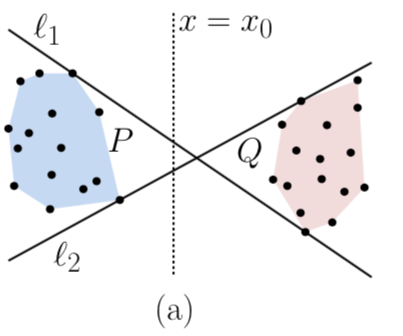
\includegraphics[width = 0.5\textwidth]{lp_a.png}
\end{figure}

\hrule


We use two LP's in successon (one to find each line).

Our first line:



\begin{align*}
  \text{Objective: }\, & & \\
  & \max m & \\
  \text{Subject To:} & & \\
  & p_i.x \cdot m + b \geq p_i.y & \forall p_i \in P \\
  & q_i.x \cdot m + b \leq q_i.y & \forall q_i \in Q \\
\end{align*}

The first constraint ensures that every point in $P$ is below the line ($y = mx + b$)
Since $(x, y) \leq \ell_1 \implies y \leq \ell_1(x) = m x + b$.
The second constant ensures that every point in $Q$ is above the line.
This LP finds the negative sloping line ($\ell_1$), so we want to choose the one with the least negative slope,
aka maximize the slope.

The second LP is almost identical except for flipping inequalities

\begin{align*}
  \text{Objective: }\, & & \\
  & \min m & \\
  \text{Subject To:} & & \\
  & p_i.x \cdot m + b \leq p_i.y & \forall p_i \in P \\
  & q_i.x \cdot m + b \geq q_i.y & \forall q_i \in Q \\
\end{align*}

The first constraint ensures that every point in $P$ is above the line.
and the second constant ensures that every point in $Q$ is below the line.
This LP finds the positive sloping line ($\ell_2$), so we want the line with the least positive slope,
aka minimizing the slope.

We note that $m, b$ are unknowns, so the search-space is $m, b$ plane in $\reals ^2$.
So the resulting optimal point from our LP's is a point $(m,b)$, which we translate into line $y = mx + b$

\textbf{Running Time:} The (expected) running time is determined by the number of constraints. 
There are $n$ different constraints of the form: $p_i.x \cdot m + b \geq p_i.y$ one for each $p_i$,
and similarly $m$ different constraints of the form: $q_i.x \cdot m + b \leq q_i.y$ one for each $q_i$.
Thus there are a total of $n + m$ constraints. So we can solve each LP in expected $O(n+m)$ time.

\textbf{Correctness:}

We only prove the correctness of the first LP as the second follows from the proof of the first.

\begin{proof} By Contradiction

  Suppose not, suppose that the line ($\ell_1$) is not a supporting tangent. By our constraints,
  the line returned must be supporting. Otherwise it violates constraint 1 or 2.
  Then there must be another line $\ell '$ such that $\ell ' = m' x + b'$ and $m' > m$. A contradiction,
  since we found the line with maximum slope.
\end{proof}

Thus we find two supporting tangents of $P, Q$ and our algorithm is correct.



\problem{2.2}

You have a cannon in $\reals^2$. It has three controls labeled ``a'' ``b,''
and ``c''. A projectile shot from this cannon travels along the
parabolic arc $y = a + bx - cx^2$. You are asked to determine whether it
is possible to adjust the controls so that the projectile travels above
a set of $n$ building tops, represented by a point set $P = \{p_1,
\ldots , p_n\}$ and beneath a set of $m$ floating balloons, represented
by a point set $Q = \{q_1, \ldots , q_m\}$ (see Fig. b)). Your algorithm
should run in time $O(n + m)$. (I do not care where the cannon is
actually located. If your solution is based on some assumption about the
cannon's location, please state this.)

\begin{figure}[h]
  \centering
  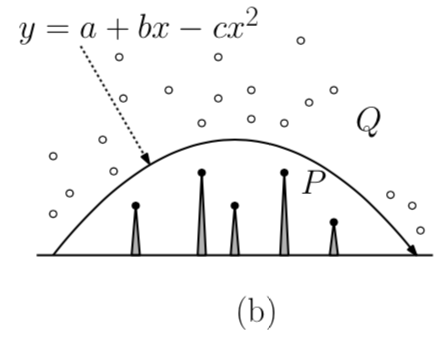
\includegraphics[width = 0.5\textwidth]{lp_b.png}
\end{figure}

\hrule

We first do some pre-processing of the points to map them into $\reals ^4$.
$p = (u,v) \in P \to p' = (x, y, z, v) \in P'$ where $p' = (1, u, u^2, v)$. \\
And similarly for $Q$ $q = (u,v) \in Q \to q' = (x, y, z, v) \in Q'$ where $q' = (1, u, u^2, v)$. 

We then build linear program:

\begin{align*}
  \text{Objective: }\, & & \\
  & \min 1 & \\
  \text{Subject To:} & & \\
  & p_i.x \cdot a + p_i.y \cdot b - p_i.z \cdot c \geq p_i.v & \forall p_i \in P' \\
  & q_i.x \cdot a + q_i.y \cdot b - q_i.z \cdot c \leq q_i.v & \forall q_i \in Q' \\
\end{align*}

Where each constraint is a halfplane in $\reals^3$ with variables $(a,b,c)$. 
The first constraint ensures that $P \leq parabola$ and the second constraint ensures 
that $Q \geq parabola$. We show this $P \leq parabola \implies v \leq parabola(u) = a \cdot (1) + b \cdot u - c \cdot u^2$.
Which by our mapping is $p.v \leq a \cdot p.x + b \cdot p.y - c \cdot p.z$.

We do not care which parabola we choose, so our objective function is just a placeholder
that will choose any feasible solution. 
The search space is $(a,b,c) \in \reals ^3$ which correspond to parabola $y = a + bx - cx^2$.

If the LP fails (empty feasible region) then we know that it is not possible to avoid all the balloons
and buildings. If it returns a value, then the feasible region is non-empty and it is possible to avoid
hitting balloons and buildings by setting proper $a, b, c$ parameters.
It should be noted, that since the algorithm returns values on the edges of the search space,
the point returned will just barely clip a balloon/building. We can change the parameters slightly
to avoid this, unless the feasible region is just a single point (lower bound of $Q$ and upper of $P$ lie on one parabola).


\textbf{Running Time:} There are a total of $m + n$ constraints, since there is one for each point in $P$ and $Q$.
Thus we can solve the LP in expected $O(n)$ time.

\textbf{Correctness: } We already showed that by our mapping a point is below the parabola
if $p.v \leq a \cdot p.x + b \cdot p.y - c \cdot p.z$ (and opposite for above). 
Constraint 1 ensures that all $P \leq parabola$ and constraint 2 ensures that all $Q \geq parabola$.
Thus if the algorithm finds a solution, it must be a valid solution that avoids all the balloons and buildings.


\problem{2.3}

You are given a set of $n$ halfplanes $H = \{h_1,\ldots,h_n\}$, where
$h_i$ is given as a pair $(a_i,b_i)$ and it consists of all the points
of the plane that lie on or beneath the line $y = a_ix + b_i$. Compute
the axis-parallel square of the largest side length whose lower edge
lies on the x-axis (see Fig.~c). If no such square exists, your
algorithm should indicate this.

\begin{figure}[h]
  \centering
  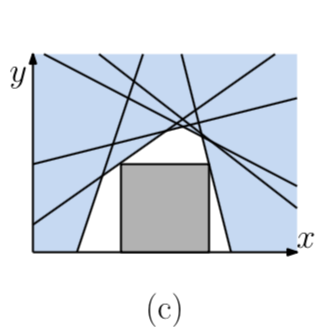
\includegraphics[width = 0.5\textwidth]{lp_c.png}
\end{figure}

\hrule





\end{document}